% 原书PDF第70页4.5起至第76页4.5.2.2之前。
\section{有向图与基因调控网络}

前面研究了基因调控的无向图模型，但无向图缺乏语义上的可解释性。有向边具有自然的因果含义，因此有向图是调控网络建模的有力工具。本节主要介绍基于评分的线性与非线性因果推断方法，用微阵列或 RNA-seq 测得的表达数据构建基因调控网络，以更深入地理解调控机制，并推断网络中的调控方向。

\subsection{推断全基因组调控网络的一般过程}
现有多数因果推断方法只能估计包含数十至数百节点的有向无环图，无法构建全基因组调控网络。不完整的调控网络图谱限制了对复杂性状与人类疾病分子机制的理解（Barzel and Barabási 2013）。基因组技术快速进步，使我们有望获得完整的全基因组调控网络，因此迫切需要发展相应的推断工具。

图4.19概括了一般过程（Liu et al. 2016），包含四个主要部分：（1）构建调控网络的初始有向无环图（DAG）；（2）为构建 DAG 选择节点集合；（3）构建因果子网络（DAG）；（4）将多个因果子网络整合为连通的因果网络。重复步骤（2）—（4），直到所推断网络的结构收敛，以最终因果网络作为全基因组调控网络。四个部分简述如下。
\begin{figure}[htbp]
\centering
\begin{tikzpicture}[x=1cm,y=1cm,>=Stealth,font=\small]
\node[rounded corners=4pt,fill=green!55!yellow!70,text=magenta!80!black,minimum width=4.8cm,minimum height=1.1cm,font=\bfseries] (ch04a19init) at (4.7,8.7) {初始网络};
\node[rounded corners=4pt,fill=green!55!yellow!70,text=magenta!80!black,minimum width=4.8cm,minimum height=1.1cm,font=\bfseries] (ch04a19select) at (4.7,7.3) {为子网络选择节点};
\node[rounded corners=4pt,fill=green!55!yellow!70,text=magenta!80!black,minimum width=4.8cm,minimum height=1.1cm,font=\bfseries] (ch04a19infer) at (4.7,5.9) {推断因果子网络};
\node[rounded corners=4pt,fill=green!55!yellow!70,text=magenta!80!black,minimum width=4.8cm,minimum height=1.1cm,font=\bfseries] (ch04a19merge) at (4.7,4.5) {整合因果子网络};
\node[rounded corners=4pt,fill=green!55!yellow!70,text=magenta!80!black,minimum width=4.8cm,minimum height=1.1cm,font=\bfseries] (ch04a19check) at (4.7,3.1) {检查结构是否收敛};
\node[ellipse,fill=green!55!yellow!70,text=magenta!80!black,minimum width=3.6cm,minimum height=.8cm,font=\bfseries] (ch04a19stop) at (4.7,1.7) {停止};
\draw[red,->] (ch04a19check.south)--node[right,text=black]{是}(ch04a19stop.north);
\draw[red,->] (ch04a19check.west)--node[above,text=black]{否}(1,3.1)--(1,7.3)--(ch04a19select.west);
\draw[red] (7.35,7.75)--(7.65,7.75)--(7.65,5.2)--(7.95,5.2)--(7.65,5.2)--(7.65,2.65)--(7.35,2.65);
\node[anchor=west,align=left,font=\bfseries] at (8.1,5.2) {网络构建\\的迭代过程};
\end{tikzpicture}
\origfig{19}{构建大规模调控网络的一般过程。}
\label{fig:ch04a-19}
\end{figure}


\par\medskip\noindent\textbf{步骤1：构建初始网络。}
初始网络可为无向或有向网络。初始无向网络可由相关和互信息（mutual information，MI）推断（Liu et al. 2016）；初始有向网络则可用基于网络评分的整数规划（第2.6节），或用于双变量因果发现的函数模型（第2.5.1.1节）构建。

\par\medskip\noindent\textbf{步骤2：选择度为 $d$ 的节点作为子网络中心节点。}
对每个中心节点，选择与其最短路径长度不超过 $k$ 的节点。中心节点与所选节点组成一个局部子网络的节点集。假设共选出 $l$ 个节点集，则可推断 $l$ 个局部子网络。

\par\medskip\noindent\textbf{步骤3：构建局部子网络。}
对每个所选节点集，采用 DAG 推断算法构建局部子网络。例如，用稀疏结构方程模型计算每个节点的评分函数，再用整数规划算法选择评分最优的局部网络，共构建 $l$ 个子网络。

\par\medskip\noindent\textbf{步骤4：整合局部因果子网络。}
取全部局部因果子网络的并集，将它们整合为连通的全局网络。若不同局部网络给出的方向不同，则用双变量因果发现的函数模型确定方向。该步骤输出暂定的全局调控网络。重复步骤2—4，直到网络拓扑结构收敛。

\subsection{用于全基因组调控网络的层次贝叶斯网络}
基因表达谱通常测量大量基因，现有 DAG 构建算法无法联合构建全基因组调控网络。本节介绍层次贝叶斯网络（hierarchical Bayesian network）建模方法（图4.20），它也可用于第4.5.1节讨论的初始调控网络。

层次贝叶斯网络推断包括三个步骤。第一，确定用于生成子网络的节点（基因）集合。若一些基因在通路数据库中组成一条通路，则以该通路的全部基因为一组，构建局部因果子网络。许多基因未收录于通路数据库，可通过聚类分析将它们分组，以每个簇的基因为一组推断局部子网络。随后，用 PCA、矩阵补全等汇总统计量表示每组全部基因的表达，基于各组的汇总统计量，用基于评分的整数规划推断组间表达因果关系的 DAG。第二，用基于评分的整数规划方法构建局部调控网络。第三，将全部调控子网络整合为连通的全基因组调控网络。
\begin{figure}[htbp]
\centering
\begin{tikzpicture}[x=1cm,y=1cm,>=Stealth,font=\small]
\node[draw=inkblue,rounded corners=7pt,minimum width=4.2cm,minimum height=2.35cm] (ch04a20abox) at (2.1,5.5) {};
\node[circle,fill=red!85,inner sep=0,minimum size=.25cm] (ch04a20a1) at (0.65,6.300000000000001) {};
\node[circle,fill=red!85,inner sep=0,minimum size=.25cm] (ch04a20a2) at (0.9,5.300000000000001) {};
\node[circle,fill=red!85,inner sep=0,minimum size=.25cm] (ch04a20a3) at (2.1,6.25) {};
\node[circle,fill=red!85,inner sep=0,minimum size=.25cm] (ch04a20a4) at (2,4.9) {};
\node[circle,fill=red!85,inner sep=0,minimum size=.25cm] (ch04a20a5) at (3,6.2) {};
\node[circle,fill=red!85,inner sep=0,minimum size=.25cm] (ch04a20a6) at (3.4,5.2) {};
\draw[->,magenta] (ch04a20a1)--(ch04a20a2);
\draw[->,magenta] (ch04a20a3)--(ch04a20a2);
\draw[->,magenta] (ch04a20a2)--(ch04a20a4);
\draw[->,magenta] (ch04a20a5)--(ch04a20a4);
\draw[->,magenta] (ch04a20a5)--(ch04a20a6);
\node[draw=inkblue,rounded corners=7pt,minimum width=4.2cm,minimum height=2.35cm] (ch04a20bbox) at (10.299999999999999,5.5) {};
\node[circle,fill=red!85,inner sep=0,minimum size=.25cm] (ch04a20b1) at (8.85,6.300000000000001) {};
\node[circle,fill=red!85,inner sep=0,minimum size=.25cm] (ch04a20b2) at (9.1,5.300000000000001) {};
\node[circle,fill=red!85,inner sep=0,minimum size=.25cm] (ch04a20b3) at (10.299999999999999,6.25) {};
\node[circle,fill=red!85,inner sep=0,minimum size=.25cm] (ch04a20b4) at (10.2,4.9) {};
\node[circle,fill=red!85,inner sep=0,minimum size=.25cm] (ch04a20b5) at (11.2,6.2) {};
\node[circle,fill=red!85,inner sep=0,minimum size=.25cm] (ch04a20b6) at (11.6,5.2) {};
\draw[->,magenta] (ch04a20b1)--(ch04a20b2);
\draw[->,magenta] (ch04a20b3)--(ch04a20b2);
\draw[->,magenta] (ch04a20b2)--(ch04a20b4);
\draw[->,magenta] (ch04a20b5)--(ch04a20b4);
\draw[->,magenta] (ch04a20b5)--(ch04a20b6);
\node[draw=inkblue,rounded corners=7pt,minimum width=4.2cm,minimum height=2.35cm] (ch04a20cbox) at (1.6,2.8) {};
\node[circle,fill=red!85,inner sep=0,minimum size=.25cm] (ch04a20c1) at (0.15000000000000002,3.5999999999999996) {};
\node[circle,fill=red!85,inner sep=0,minimum size=.25cm] (ch04a20c2) at (0.4,2.6) {};
\node[circle,fill=red!85,inner sep=0,minimum size=.25cm] (ch04a20c3) at (1.6,3.55) {};
\node[circle,fill=red!85,inner sep=0,minimum size=.25cm] (ch04a20c4) at (1.5,2.2) {};
\node[circle,fill=red!85,inner sep=0,minimum size=.25cm] (ch04a20c5) at (2.5,3.5) {};
\node[circle,fill=red!85,inner sep=0,minimum size=.25cm] (ch04a20c6) at (2.9,2.5) {};
\draw[->,magenta] (ch04a20c1)--(ch04a20c2);
\draw[->,magenta] (ch04a20c3)--(ch04a20c2);
\draw[->,magenta] (ch04a20c2)--(ch04a20c4);
\draw[->,magenta] (ch04a20c5)--(ch04a20c4);
\draw[->,magenta] (ch04a20c5)--(ch04a20c6);
\node[draw=inkblue,rounded corners=7pt,minimum width=4.2cm,minimum height=2.35cm] (ch04a20dbox) at (10.6,2.8) {};
\node[circle,fill=red!85,inner sep=0,minimum size=.25cm] (ch04a20d1) at (9.15,3.5999999999999996) {};
\node[circle,fill=red!85,inner sep=0,minimum size=.25cm] (ch04a20d2) at (9.4,2.6) {};
\node[circle,fill=red!85,inner sep=0,minimum size=.25cm] (ch04a20d3) at (10.6,3.55) {};
\node[circle,fill=red!85,inner sep=0,minimum size=.25cm] (ch04a20d4) at (10.5,2.2) {};
\node[circle,fill=red!85,inner sep=0,minimum size=.25cm] (ch04a20d5) at (11.5,3.5) {};
\node[circle,fill=red!85,inner sep=0,minimum size=.25cm] (ch04a20d6) at (11.9,2.5) {};
\draw[->,magenta] (ch04a20d1)--(ch04a20d2);
\draw[->,magenta] (ch04a20d3)--(ch04a20d2);
\draw[->,magenta] (ch04a20d2)--(ch04a20d4);
\draw[->,magenta] (ch04a20d5)--(ch04a20d4);
\draw[->,magenta] (ch04a20d5)--(ch04a20d6);
\node[draw=inkblue,rounded corners=7pt,minimum width=4.2cm,minimum height=2.35cm] (ch04a20ebox) at (6.199999999999999,1.1) {};
\node[circle,fill=red!85,inner sep=0,minimum size=.25cm] (ch04a20e1) at (4.75,1.9) {};
\node[circle,fill=red!85,inner sep=0,minimum size=.25cm] (ch04a20e2) at (5.0,0.9) {};
\node[circle,fill=red!85,inner sep=0,minimum size=.25cm] (ch04a20e3) at (6.199999999999999,1.85) {};
\node[circle,fill=red!85,inner sep=0,minimum size=.25cm] (ch04a20e4) at (6.1,0.5) {};
\node[circle,fill=red!85,inner sep=0,minimum size=.25cm] (ch04a20e5) at (7.1,1.8) {};
\node[circle,fill=red!85,inner sep=0,minimum size=.25cm] (ch04a20e6) at (7.5,0.8) {};
\draw[->,magenta] (ch04a20e1)--(ch04a20e2);
\draw[->,magenta] (ch04a20e3)--(ch04a20e2);
\draw[->,magenta] (ch04a20e2)--(ch04a20e4);
\draw[->,magenta] (ch04a20e5)--(ch04a20e4);
\draw[->,magenta] (ch04a20e5)--(ch04a20e6);
\draw[->,green!65!black] (ch04a20abox)--(ch04a20cbox);
\draw[->,green!65!black] (ch04a20bbox)--(ch04a20cbox);
\draw[->,green!65!black] (ch04a20bbox)--(ch04a20dbox);
\draw[->,green!65!black] (ch04a20cbox)--(ch04a20ebox);
\draw[->,green!65!black] (ch04a20dbox)--(ch04a20ebox);
\node[text=inkblue,font=\bfseries] (ch04a20pathlabel) at (5.3,6.95) {通路};
\draw[->,inkblue] (ch04a20abox.east)--(ch04a20pathlabel);
\node[text=red,font=\bfseries] (ch04a20genelabel) at (11.3,.7) {基因};
\draw[->,red] (ch04a20d4)--(ch04a20genelabel);
\end{tikzpicture}
\origfig{20}{初始贝叶斯网络示意图。}
\label{fig:ch04a-20}
\end{figure}


\subsubsection{表示基因表达组的汇总统计量}
广义低秩模型包括矩阵补全（根据低秩矩阵中不完整的条目填补缺失值）、PCA 与稳健 PCA（从受污染的矩阵恢复原始低秩矩阵）（Liu et al. 2013；Udell et al. 2016；Candès et al. 2009）。这些模型能有效降低数据维数、分割（聚类）数据，并汇总通路或簇中的基因表达。本节主要介绍低秩矩阵表示模型，将稳健 PCA 视为其特例。

考虑具有 $d$ 行、$n$ 个样本的观测基因表达矩阵 $X\in\mathbb R^{d\times n}$。对于微阵列数据，每行表示一个基因在 $n$ 个样本中的表达。对于 RNA-seq 数据，若以总体表达水平汇总基因区域的表达，则每行同样表示一个基因在全部样本中的表达。RNA-seq 数据也可按函数主成分展开，用多个主成分得分表示一个基因的表达，此时矩阵 $X$ 包含这些得分，每行由某一基因的一个函数主成分在 $n$ 个样本中的得分组成。假设受噪声污染的 $X$ 可分解为（图4.21）
\begin{equation}
X=AZ+E,
\tag{4.150}
\end{equation}
其中 $A\in\mathbb R^{n\times r}$ 为线性张成数据空间的“字典”矩阵，$Z\in\mathbb R^{r\times n}$ 为表达数据矩阵 $X$ 相对于字典 $A$ 的最低秩表示，$E\in\mathbb R^{d\times n}$ 为噪声矩阵。目标是去除噪声 $E$，恢复原始低秩矩阵 $X_0$，其中
\begin{equation}
X=X_0+E.
\tag{4.151}
\end{equation}
式 (4.151) 表明，原始低秩矩阵 $X_0$ 受噪声污染后产生观测矩阵 $X$。
\begin{figure}[htbp]
\centering
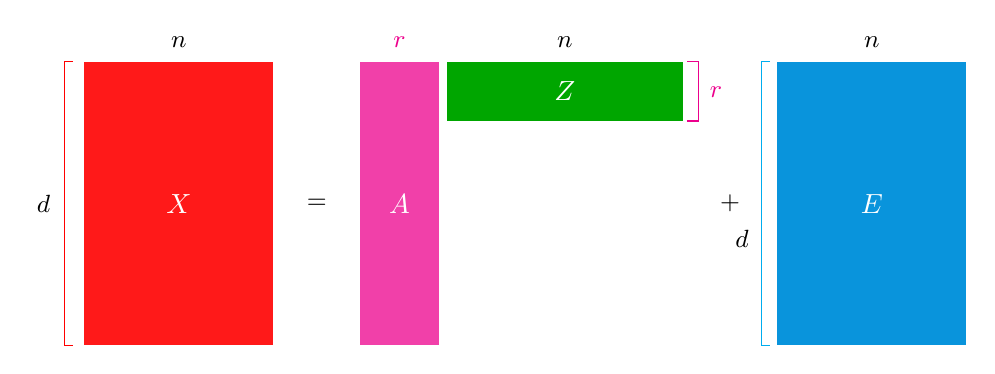
\begin{tikzpicture}[x=1cm,y=1cm,font=\small]
\fill[red!90] (.6,0) rectangle (3,3.6);
\fill[magenta!75] (4.1,0) rectangle (5.1,3.6);
\fill[green!65!black] (5.2,2.85) rectangle (8.2,3.6);
\fill[cyan!80!blue] (9.4,0) rectangle (11.8,3.6);
\node[text=white,font=\bfseries] at (1.8,1.8) {$X$};
\node[text=white,font=\bfseries] at (4.6,1.8) {$A$};
\node[text=white,font=\bfseries] at (6.7,3.23) {$Z$};
\node[text=white,font=\bfseries] at (10.6,1.8) {$E$};
\node at (3.55,1.8) {$=$};\node at (8.8,1.8) {$+$};
\node at (1.8,3.85) {$n$};\node[text=magenta] at (4.6,3.85) {$r$};
\node at (6.7,3.85) {$n$};\node at (10.6,3.85) {$n$};
\draw[red] (.45,0)--(.35,0)--(.35,3.6)--(.45,3.6);\node at (.08,1.8) {$d$};
\draw[magenta] (8.25,2.85)--(8.4,2.85)--(8.4,3.6)--(8.25,3.6);\node[text=magenta] at (8.62,3.22) {$r$};
\draw[cyan] (9.3,0)--(9.2,0)--(9.2,3.6)--(9.3,3.6);\node at (8.95,1.35) {$d$};
\end{tikzpicture}
\origfig{21}{低秩模型。}
\label{fig:ch04a-21}
\end{figure}

上述目标可通过下列优化实现：
\begin{equation}
\begin{aligned}
\min_{Z,E}\quad&\lVert Z\rVert_*+\lambda\lVert E\rVert_{2,1}\\
\text{s.t.}\quad&X=AZ+E,
\end{aligned}
\tag{4.152}
\end{equation}
其中 $\lVert\cdot\rVert_*$ 表示核范数，即矩阵奇异值之和；$\lVert E\rVert_{2,1}=\sum_j\lVert[E]_{:,j}\rVert_2$，$\lVert\cdot\rVert_2$ 为 $L_2$ 范数，$[E]_{:,j}$ 为 $E$ 的第 $j$ 列；$\lambda$ 为惩罚参数。实际中常用核范数代替秩函数。这里用 $L_{2,1}$ 范数刻画误差项，惩罚 $\lambda\lVert E\rVert_{2,1}$ 旨在去除样本特异性污染造成的离群点。为去除小的高斯噪声，可采用 $\lVert E\rVert_F^2$ 惩罚；为去除随机污染，则采用 $L_1$ 范数 $\lVert E\rVert_1$。

求解问题 (4.152) 后，用 $Z^*$ 表示组内基因表达。$Z^*$ 的第 $j$ 列是含 $r$ 个分量的表示得分向量，汇总第 $j$ 个样本中组内全部基因的表达。原始低秩矩阵 $X_0$ 可由 $AZ^*$ 或 $Z-E^*$ 恢复，其中 $E^*$ 为误差矩阵的最优解。

进一步将问题转化为
\begin{equation}
\begin{aligned}
\min_{Z,E,J}\quad&\lVert J\rVert_*+\lambda\lVert E\rVert_{2,1}\\
\text{s.t.}\quad&X=AZ+E,\quad Z=J.
\end{aligned}
\tag{4.153}
\end{equation}
可用交替方向乘子法（alternating direction method of multipliers，ADMM）（Boyd et al. 2011）求解，最小化增广 Lagrange 函数
\begin{equation}
\begin{aligned}
L(Z,E,J,Y_1,Y_2,\lambda,\mu)
={}&\lVert J\rVert_*+\lambda\lVert E\rVert_{2,1}
+\operatorname{tr}(Y_1^T(X-AZ-E))\\
&+\operatorname{tr}(Y_2^T(Z-J))
+\frac\mu2(\lVert X-AZ-E\rVert_F^2+\lVert Z-J\rVert_F^2).
\end{aligned}
\tag{4.154}
\end{equation}
相应 ADMM 算法如下，详细推导见附录4.C。

\begin{bookalgorithm}{4.2：ADMM 算法}
\noindent\textbf{步骤1：初始化。}
令 $Z=J=0$、$E=0$、$Y_1=0$、$Y_2=0$、$\mu=10^{-6}$、$\mu_{\max}=10^{-6}$、$\rho=1.1$、$\varepsilon=10^{-8}$。

\noindent\textbf{步骤2：重复以下过程直到收敛。}
\begin{enumerate}[label=\alph*.,leftmargin=2em]
\item 更新 $J$。进行奇异值分解：
\[
Z^{(k)}+\frac1\mu Y_2^{(k)}=U^{(k+1)}\Sigma^{(k+1)}(V^{(k+1)})^T,
\]
其中 $\Sigma^{(k+1)}=\operatorname{diag}(\sigma_1^{(k+1)},\ldots,\sigma_r^{(k+1)})$。更新
\[
\begin{aligned}
J^{(k+1)}=U^{(k+1)}\operatorname{diag}\Bigl(
&\max(\sigma_1^{(k+1)}-1/\mu,0),\ldots,\\
&\max(\sigma_r^{(k+1)}-1/\mu,0)\Bigr)(V^{(k+1)})^T.
\end{aligned}
\]
\item 更新 $Z$：
\[
Z^{(k+1)}=(I+A^TA)^{-1}\left[A^T(X-E^{(k)})+J^{(k+1)}
+\frac1\mu(A^TY_1^{(k)}-Y_2^{(k)})\right].
\]
\item 更新 $E$。定义 $Q=X-AZ^{(k+1)}+Y_1^{(k)}/\mu$，则
\[
[E^{(k+1)}]_{:,j}
=\frac{(\lVert[Q]_{:,j}\rVert_2-\lambda/\mu)_+}{\lVert[Q]_{:,j}\rVert_2}[Q]_{:,j}.
\]
\item 更新乘子：
\[
\begin{aligned}
Y_1^{(k+1)}&=Y_1^{(k)}+\mu(X-AZ^{(k+1)}-E^{(k+1)}),\\
Y_2^{(k+1)}&=Y_2^{(k)}+\mu(Z^{(k+1)}-J^{(k+1)}).
\end{aligned}
\]
\item 更新参数 $\mu=\min(\rho\mu,\mu_{\max})$。
\item 检查收敛条件。若
\[
\lVert X-AZ^{(k+1)}-E^{(k+1)}\rVert_\infty<\varepsilon,\qquad
\lVert Z^{(k+1)}-J^{(k+1)}\rVert_\infty<\varepsilon,
\]
则停止；否则令 $k\leftarrow k+1$，返回步骤2（a）。
\end{enumerate}
\noindent 结束。
\end{bookalgorithm}

下面讨论如何用低秩表示模型分割数据。在式 (4.152) 中选择 $A=X$，问题化为
\begin{equation}
\begin{aligned}
\min_{Z,E}\quad&\lVert Z\rVert_*+\lambda\lVert E\rVert_{2,1}\\
\text{s.t.}\quad&X=XZ+E.
\end{aligned}
\tag{4.155}
\end{equation}
同样可用 ADMM 求解。得到最优解 $(Z^*,E^*)$ 后，使用下列算法分割（聚类）数据。

\begin{bookalgorithm}{4.3：子空间分割（聚类分析）算法}
\noindent\textbf{步骤1：}得到极小值点 $Z^*$，计算其薄型 SVD：$U^*\Sigma^*(V^*)^T$。

\noindent\textbf{步骤2：}构造亲和矩阵 $W$。令 $\widetilde U=U^*(\Sigma^*)^{1/2}$，则 $[W]_{ij}=([\widetilde U\widetilde U^T]_{ij})^2$。平方的目的是保证亲和矩阵取值为正，因为 $\widetilde U\widetilde U^T$ 可能有负值。

\noindent\textbf{步骤3：}以亲和矩阵 $W$ 进行 Ncut，将数据样本分为 $k$ 个簇。
\begin{enumerate}[label=\alph*.,leftmargin=2em]
\item 令 $d_i=\sum_j[W]_{ij}$，定义对角矩阵 $D=\operatorname{diag}(d_1,\ldots,d_D)$。求解特征方程
\[
(D-W)e=\lambda De,
\]
或
\[
D^{-1/2}(D-W)D^{-1/2}g=\lambda g,\qquad g=D^{-1/2}e.
\]
\item 用第二小特征值对应的特征向量二分图。具体而言，计算该特征向量 $e$ 的各分量中位数 $m$，将 $e$ 中分量大于 $m$ 的点置于簇 $G_1$，其余置于 $G_2$。重复以这种方式划分子集，实现层次聚类。
\end{enumerate}
\noindent\textbf{步骤4：}估计子空间数 $k$（簇数）：
\[
\hat k=n-\operatorname{int}\left(\sum_{i=1}^{n}f_\tau(\sigma_i)\right),
\]
其中 $\operatorname{int}(\cdot)$ 输出最接近某实数的整数；$\sigma_i$（$i=1,\ldots,n$）为拉普拉斯矩阵 $L=D-W$ 的奇异值；$0<\tau<1$ 为参数，且
\[
f_\tau(\sigma)=\begin{cases}
1,&\sigma>\tau,\\
\log_2\left(1+\dfrac{\sigma^2}{r^2}\right),&\text{其他情形。}
\end{cases}
\]
\end{bookalgorithm}
\FloatBarrier
